\documentclass[a4paper,10pt,titlepage]{article}
% Språk och encodings
\usepackage[swedish,english]{babel}
\usepackage[T1]{fontenc}
\usepackage[utf8]{inputenc}
\usepackage[fixlanguage]{babelbib}
% Images and floats
\usepackage{graphicx}
\usepackage{wrapfig}
\usepackage{float}
% Clear type + Sans-serif font
\usepackage{lmodern}
\renewcommand{\familydefault}{\sfdefault}
% Avancerade tabeller
\usepackage{tabularx}
\usepackage{multirow}
\usepackage{booktabs}
% Matte
\usepackage{amsmath, amsthm, amssymb}
% Algoritmer
\usepackage[ruled,vlined]{algorithm2e}
% Källkod
\usepackage{listings}
\lstset{
	showspaces = false,
	showstringspaces = false,
}
% Inkludera pdf-sidor
\usepackage{pdfpages}
% Länkar
\usepackage{color}
\definecolor{dark-blue}{rgb}{0, 0, 0.6}
\usepackage{hyperref}
\hypersetup{
  colorlinks=true,
  linkcolor=dark-blue,
  urlcolor=dark-blue
}
% Vettiga paragrafer
\setlength{\parindent}{0pt}
\setlength{\parskip}{2ex}

% Kommando för kommandorader
\newcommand{\cmdline}[1]{\mbox{\textbf{\texttt{> #1}}}}

% Kommandon för testfall
\usepackage{testcases}

% Sidhuvud/sidfot
\usepackage{fancyhdr}
\setlength{\headheight}{15pt}
\pagestyle{fancyplain}
\lfoot{Carl-Oscar Erneholm \\ 880422-0872 \\ coer@kth.se}
\rfoot{Martin Nycander \\ 881028-0076 \\ mnyc@kth.se}
\cfoot{Sida \thepage}

% Språk
\selectbiblanguage{swedish}
\selectlanguage{swedish}

% Titel
\title{Laborationsrapport 3 \\ Minneshantering v. 3.21}
\author{Carl-Oscar Erneholm \and Martin Nycander}
\date{\today}

\begin{document}

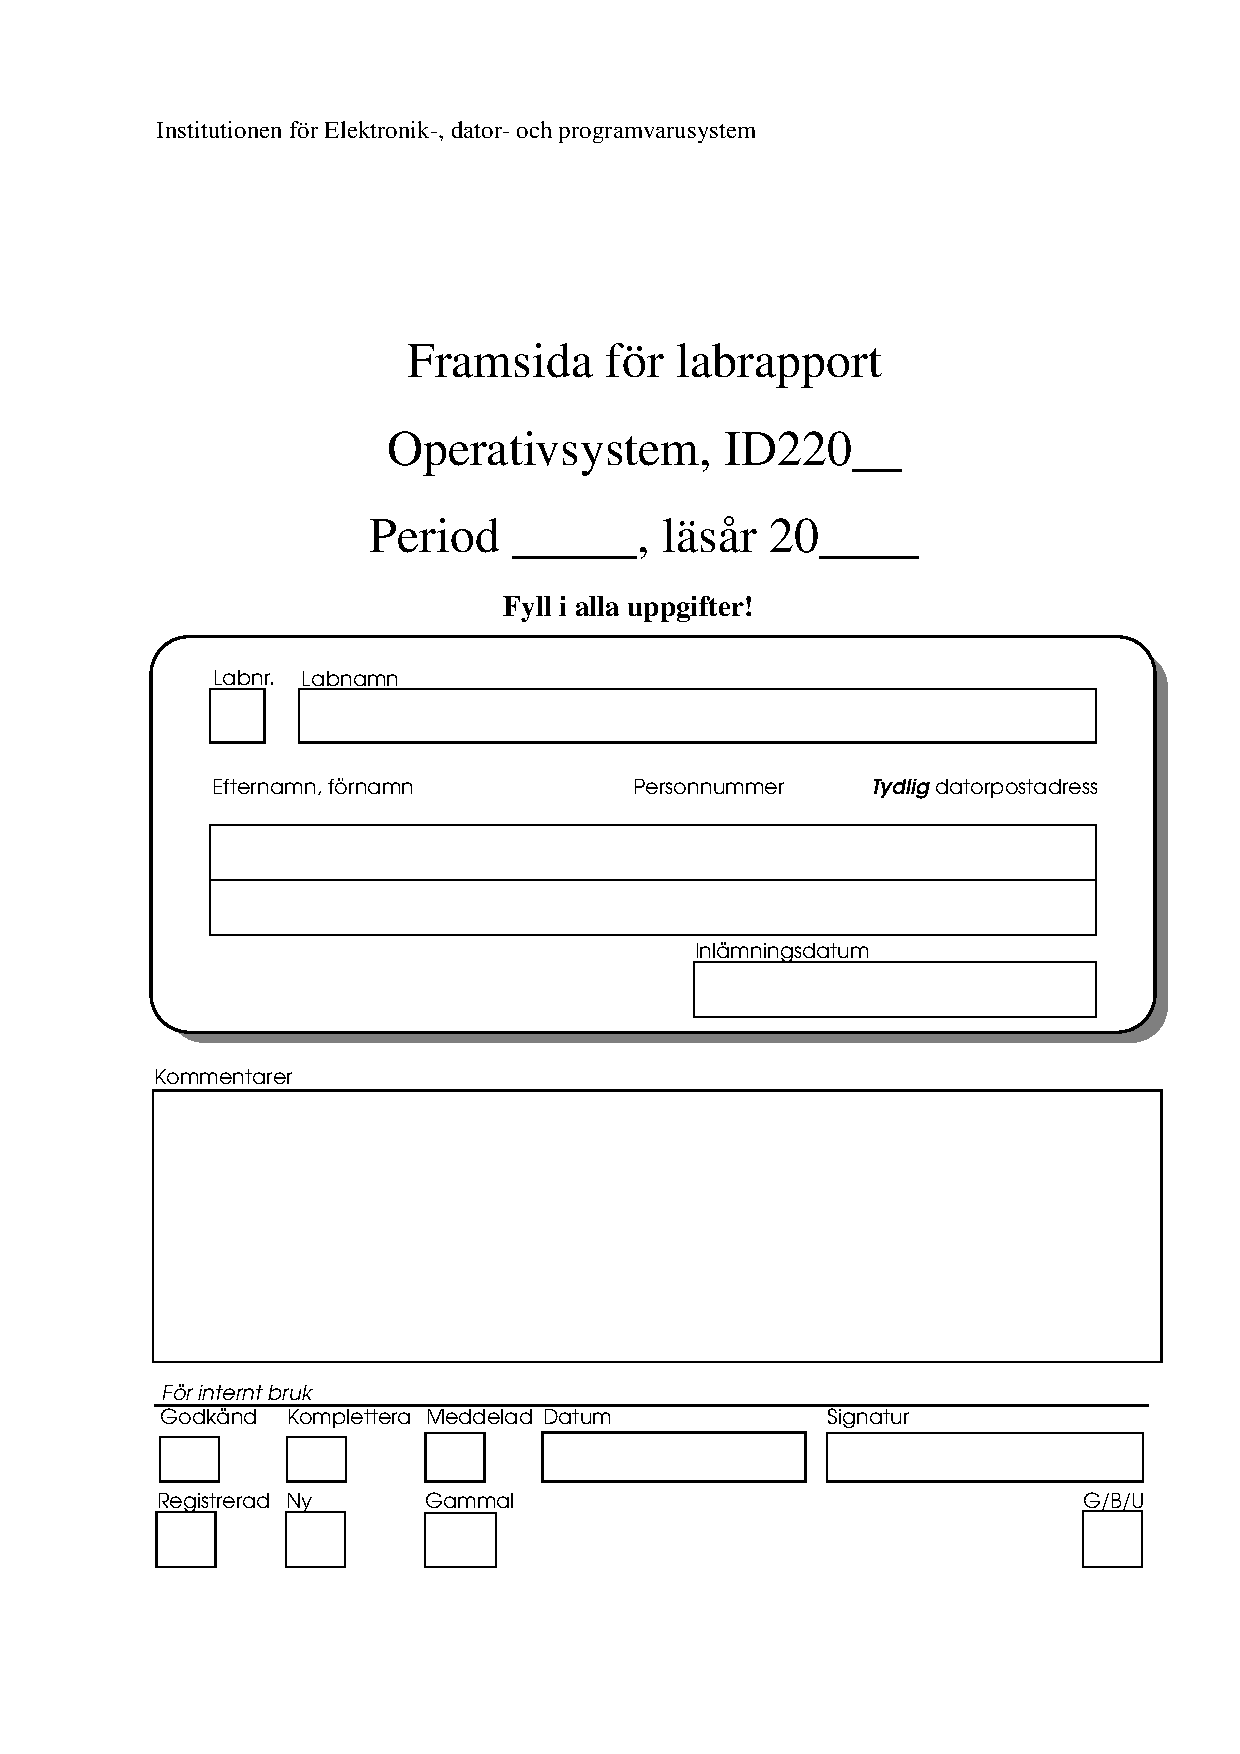
\includepdf[pages=-]{framsida.pdf}

\maketitle

\tableofcontents
\thispagestyle{empty}
\newpage
\setcounter{page}{1}
\section{Problembeskrivning}


\subsection{Förberedelsefråga}

\begin{enumerate}
	\item[1.] \textbf{\footnotesize Hur mycket minne slösas bort i medel och i värsta fallet i de block som allokeras via malloc() ur ``Quick fit'' listorna?}

	\verb!TODO!

\end{enumerate}

\newpage
\section{Programbeskrivning}

\newpage
\section{Prestandautvärdering}

% TODO: Använd testcases för att standardisera hur prestandamätningen görs

% TODO: GRAFER! PIE-CHARTS!!!!!!!!

% TODO: Noggrannhet?

\newpage
\section{Resultat}


\newpage
\section{Labbutvärdering}

\newpage

\end{document}
